\documentclass[table]{beamer}

\usepackage[british]{babel}
\usepackage{graphicx,hyperref,hit,url}
\usepackage{CJKutf8}
\usepackage{xcolor}
% The title of the presentation:
%  - first a short version which is visible at the bottom of each slide;
%  - second the full title shown on the title slide;
\title[optimal transport]{
  Optimal Transport Map Sampling}

% Optional: a subtitle to be dispalyed on the title slide


% The author(s) of the presentation:
%  - again first a short version to be displayed at the bottom;
%  - next the full list of authors, which may include contact information;
\author[Junjie Wang]{Junjie Wang}

% The institute:
%  - to start the name of the university as displayed on the top of each slide
%    this can be adjusted such that you can also create a Dutch version
%  - next the institute information as displayed on the title slide
\institute[Harbin Institute of technology]{
  Harbin Institute of technology\\ The Research Center of Aerospace Software  Engineering }

% Add a date and possibly the name of the event to the slides
%  - again first a short version to be shown at the bottom of each slide
%  - second the full date and event name for the title slide
\date{\today}

\begin{document}
\begin{CJK}{UTF8}{gbsn}

\begin{frame}[plain]
  \titlepage
\end{frame}

\begin{frame}
  \frametitle{Outline}

  \tableofcontents
\end{frame}

% Section titles are shown in at the top of the slides with the current section
% highlighted. Note that the number of sections determines the size of the top
% bar, and hence the university name and logo. If you do not add any sections
% they will not be visible.
\section{Introduction}
\begin{frame}
\begin{figure}
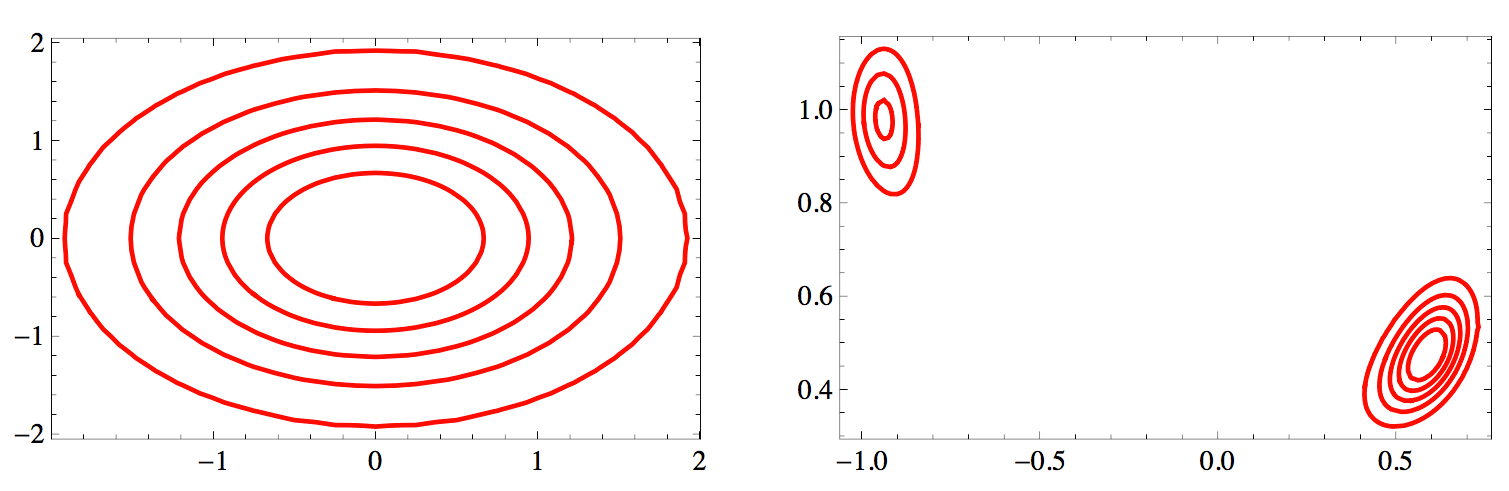
\includegraphics[scale=0.2]{img/pirorposterior1.png}
\end{figure}
\end{frame}
\begin{frame}
\begin{figure}
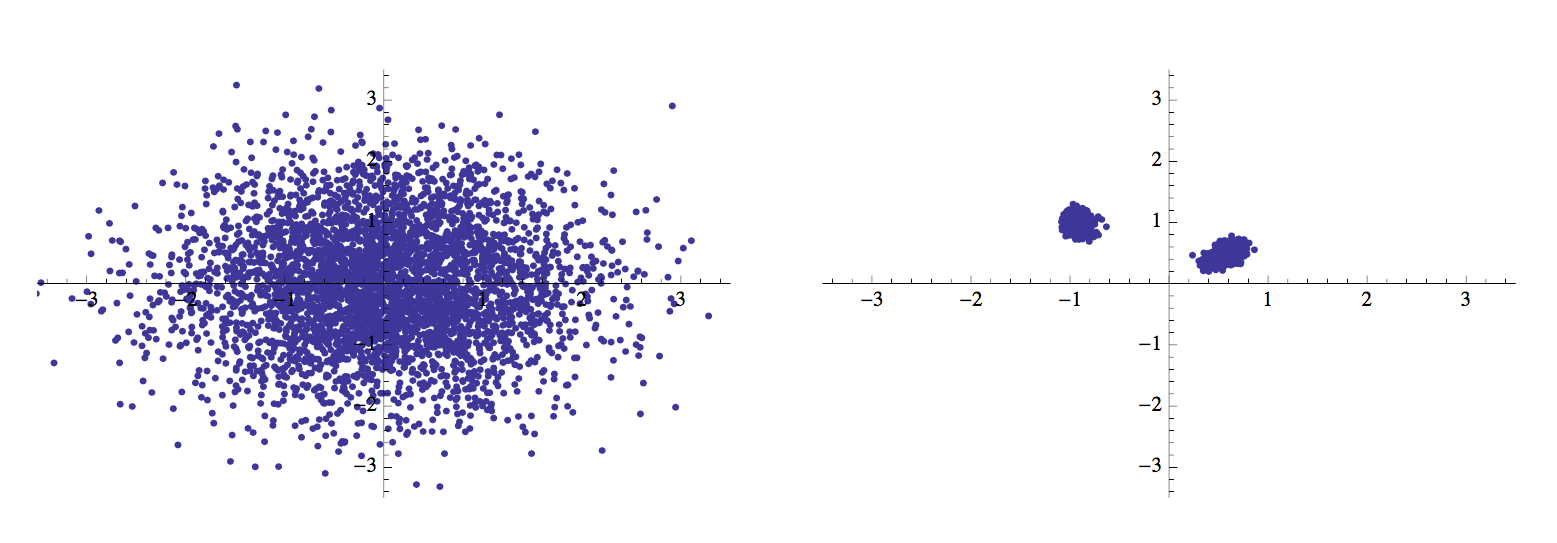
\includegraphics[scale=0.2]{img/pirorposterior2.png}
\end{figure}
Ensembles of particles represent prior pdf and posterior pdf. Compute expectations by summing over samples
\end{frame}
\begin{frame}
How to update?
\begin{figure}
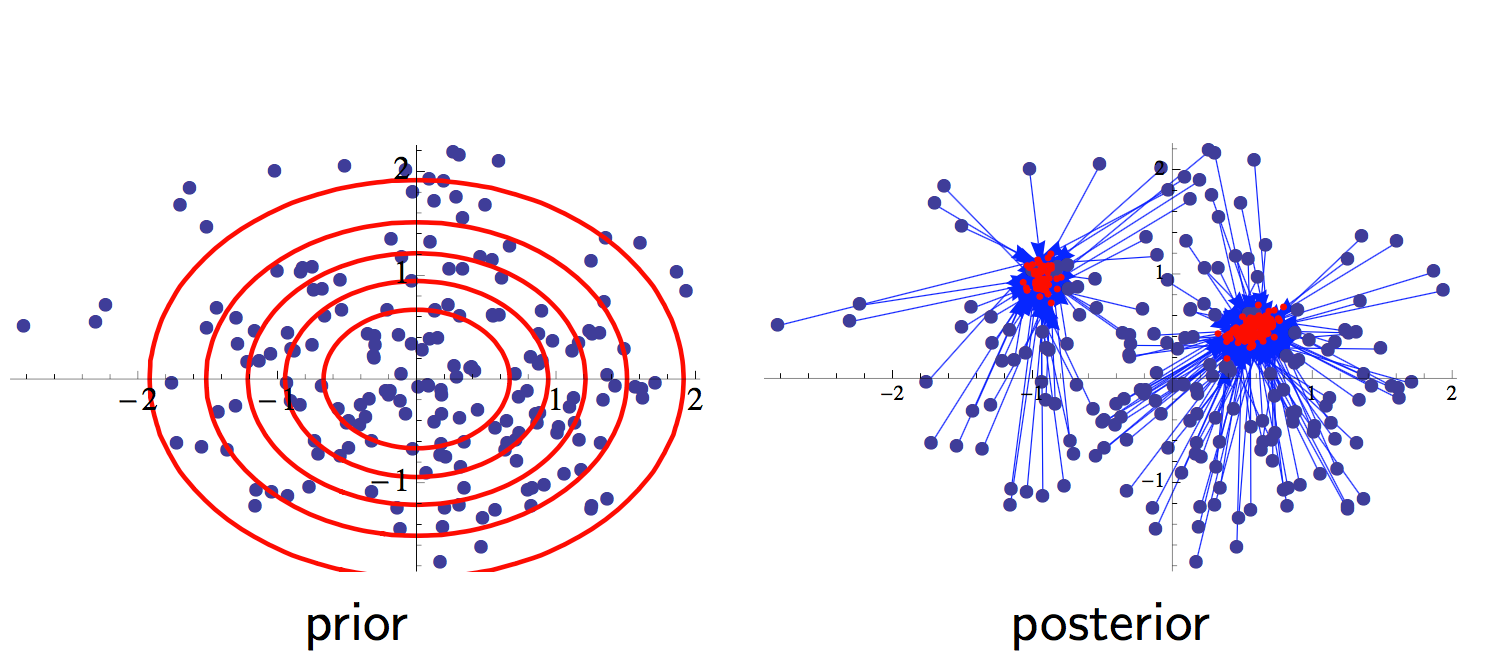
\includegraphics[scale=0.2]{img/pirorposterior3.png}
\end{figure}

\end{frame}

\begin{frame}
how to update?

\hfill

“These methods use . . . ‘samples’ that are drawn independently from the given initial distribution and assigned equal weights.
. . . When observations become available, Bayes’ rule is applied either to individual samples . . . ” (Park and Xu, 2009)

\hfill

\textbf{Note:}Bayes rule explains how to update probabilities, but not how to update samples.\\
(Particle filters do update the probability of each sample using Bayes rule.)
\end{frame}

\begin{frame}
how to update?

\hfill
\begin{itemize}
\item If prior is Gaussian and posterior is Gaussian, then any linear transformation of variables that obtains the correct posterior mean and covariance is OK.
\item when the observation operator is nonlinear?
\begin{itemize}
\item Randomized maximum likelihood (Kitanidis, 1995; Oliver et al., 1996)
\item  \textbf {Optimal map (El Moselhy and Marzouk, 2012)}
\item Implicit filters (Chorin et al., 2010; Morzfeld et al., 2012)
\item Ensemble-based iterative filters/smoothers
\end{itemize}
\end{itemize}

\end{frame}

\section{Optimal Transport Map}

\begin{frame}
  \frametitle{A different viewpoint}

\begin{figure}
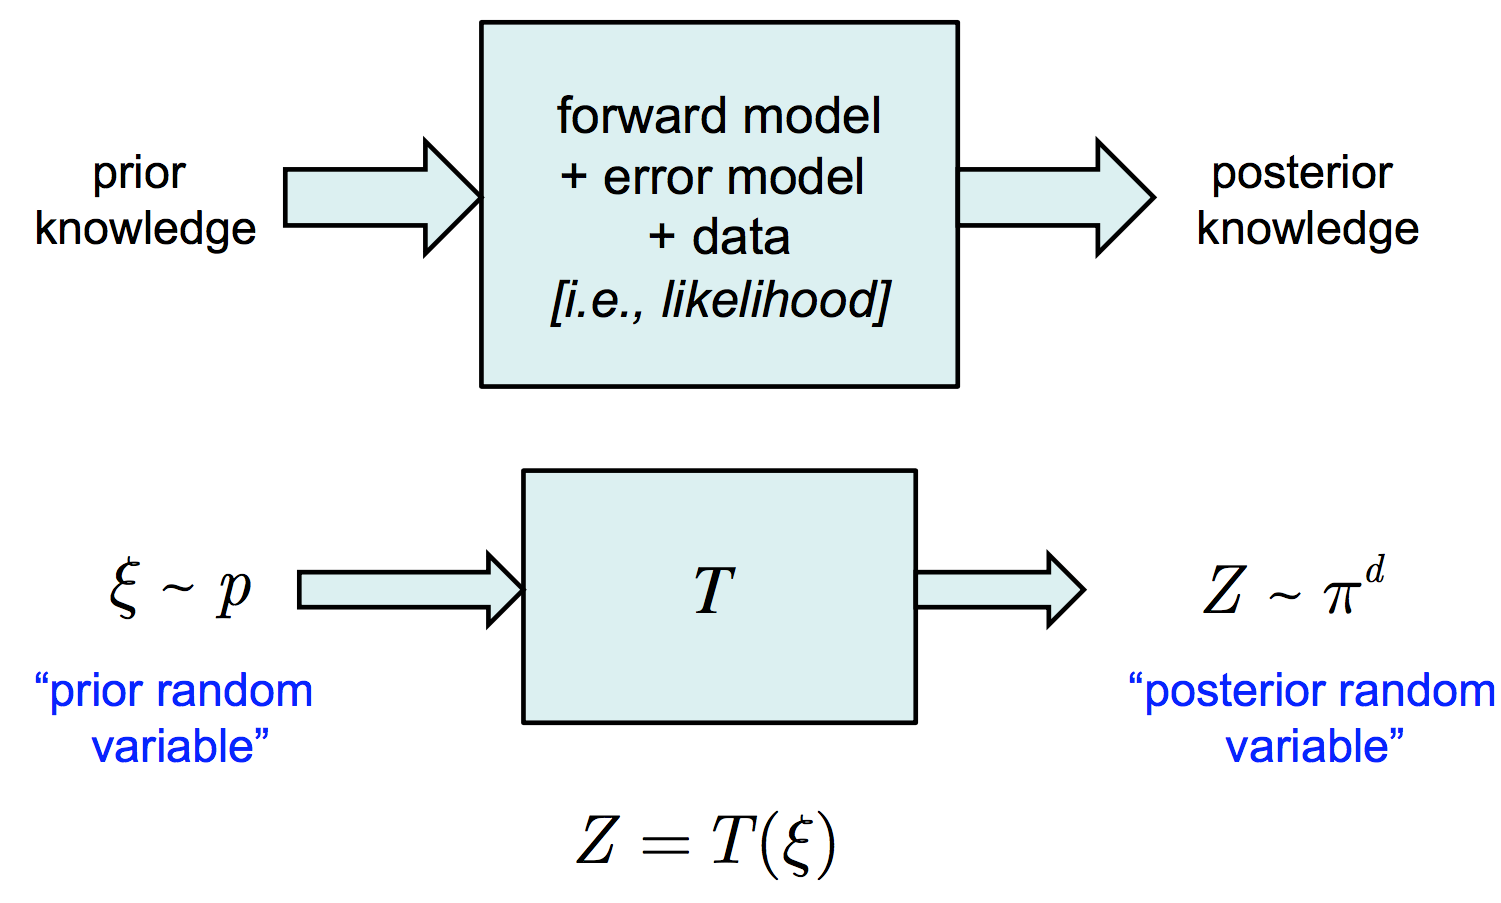
\includegraphics[scale=0.2]{img/viewpoint.png}
\end{figure}
\end{frame}


\begin{frame}
  \frametitle{Optimal transport}
Deterministic coupling of two random variables, $\xi \sim \mu, Z \sim v$
\begin{figure}
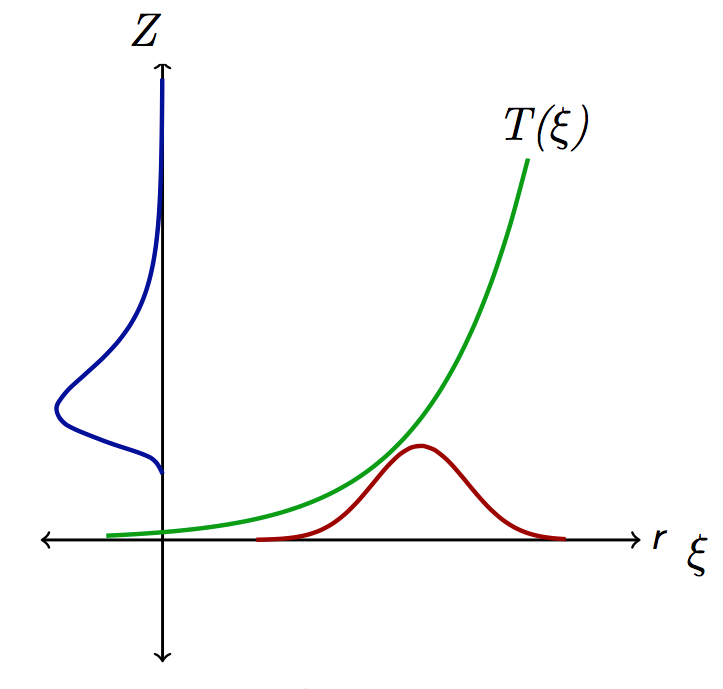
\includegraphics[scale=0.2]{img/optimaltransportmap.png}
\end{figure}

Monge problem: $\min_{T} \int c(\xi,T(\xi)) d \mu (\xi)$, where $T^{\sharp} \mu = v$
\end{frame}
\begin{frame}
  \frametitle{Optimal transport}
Let $\pi$ be the target density and $p$ be the density of a reference random variable $\xi$.
Given the ability to
\begin{itemize}
\item sample $\xi$
\item evaluate $\pi$ up to a normalizing constant
\end{itemize}
one can compute numerical approximations to the optimal map.
\hfill
The reference distribution could be the prior, or it could be something else easy to sample from
\end{frame}
\begin{frame}
\frametitle{Constructing a map}

Let $\mathcal{T}$ be an appropriate set of diffeomorhpisms. Then, any global minimizer of the optimization problem:
\begin{equation}\label{eq:minimizeropti}
\begin{aligned}
min \quad D_{KL}(T_{\sharp}\eta || \pi)\\
s.t. \quad det \nabla T > 0 \\
T \in \mathcal{T}
\end{aligned}
\end{equation}
In fact, any global minimizer of (\ref{eq:minimizeropti}) achieves the minimum cost $D_{KL}(T_{\sharp}\eta || \pi)=0$ and implies that $T_{\sharp}\eta = \pi$. The constraint det $\nabla T >0$ ensures that the pushforward density $T_{\sharp}\eta$ is strictly postive on the support of the target.
\end{frame}

\begin{frame}
\frametitle{Various types of transport}
\begin{itemize}
\item \textbf{Optimal transport:}
Monge problem: $\min_{T} \int c(\xi,T(\xi)) d \mu (\xi)$, where $T^{\sharp} \mu = v$(1781) \\
many nice properties, but numericallt challengin in general cases
\item \textbf{ Knothe-Rosenblatt rearrangement}
\begin{figure}
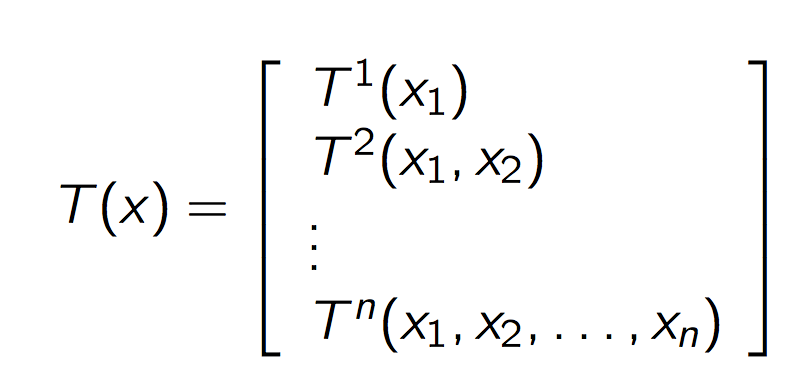
\includegraphics[scale=0.2]{img/krrearrangement.png}
\end{figure}
\begin{itemize}
  \item Exists and is unique (up to ordering) under mild conditions
  \item Jacobian determinant easy to evaluate
\end{itemize}
\end{itemize}
\end{frame}
\begin{frame}
\frametitle{Other possible transports:}
\begin{figure}
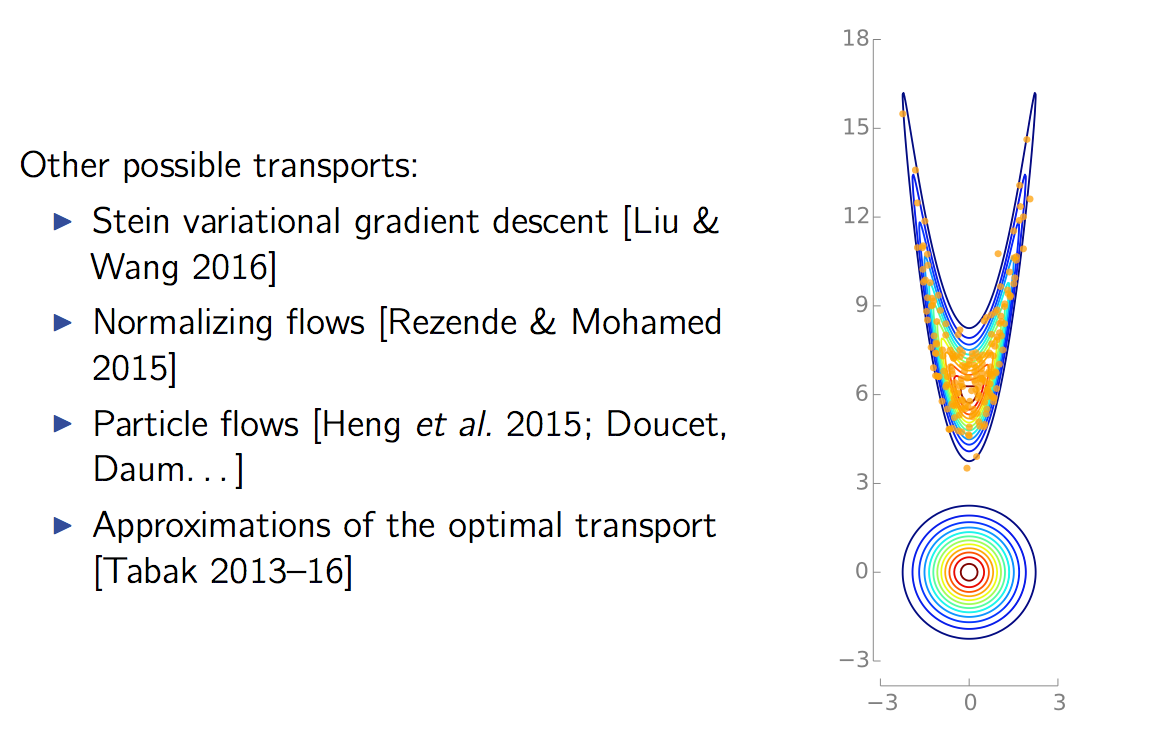
\includegraphics[scale=0.3]{img/othertransport.png}
\end{figure}
\end{frame}
\begin{frame}
\frametitle{Potential advantages}
\begin{itemize}
\item Move samples; don’t just reweigh them
\item Use optimization to enhance integration
\item Independent, unweighted, and cheap samples from the target (or
close to it
\item Clear convergence criterion, even with unnormalized target density
\item high-dimensional sampling
\end{itemize}

\end{frame}
\section{Relation to the Particle Filter}
\subsection{Relation to the particle flow filter}
\begin{frame}
\frametitle{Relation with PFF}
"We emphasize that our flow is not KnotheRosenblatt
transport, but rather it is a completely different
algorithm for particle flow."

\hfill

\begin{thebibliography}{1}
\beamertemplatearticlebibitems
\bibitem{particleflow2013daum} Particle flow inspired by Knothe-Rosenblatt
transport for nonlinear filters

\bibitem{particleflow2012daum} Particle flow and Monge-Kantorovich transport
\end{thebibliography}

\end{frame}

\begin{frame}
\frametitle{Relation with PFF}
The particle flow filter is similar with the Monge-Kantorovich optimal transport(MKT) algorithms. But they differ in \textcolor{blue}{computational complexity and the overall intendend purpose}.(Fred Daum \& Jim Huang )


\begin{tabular}{|r|r|r|}
\hline
methods & PFF & MTK\\
\hline
purpose & fix the particle degenercy & transform   particles  \\
computational & fast & slow \\
dimension & high  & \textcolor{red}{low} \\
approach & log-homotopy & \textcolor{red}{homotopy} \\
\hline
\end{tabular}

\end{frame}

\begin{frame}
\frametitle{Relation with PFF}
 In contrast to MKT, for nonlinear
filters, we are not interested in transporting physical
objects or minimizing anything related to work or effort or
energy or anything physical, but rather we merely want to
move our particles from the prior density to the posteriori
density with a small computational complexity. This is
exactly what Knothe-Rosenblatt transport (KRT) tries to
do!

\hfill

\textbf{ Unfortunately, despite the reduced computational complexity of KRT, it
is still too much for high dimensional nonlinear filter
problems. }

\end{frame}

\subsection{Coupling Particle Filter}
\begin{frame}
\frametitle{Coupling Particle filter}
Although the optimal mass transport problem has many desirable properties it
also has drawbacks. Monge’s formulation is a \textcolor{blue}{nonconvex optimization problem} and
the Kantorovich formulation results in \textcolor{blue}{large-scale optimization problems}.
A recent development to address this computational problem builds on adding
an entropic barrier term and solving the resulting optimization problem using the
so called \textcolor{red}{Sinkhorn iterations}.
\begin{thebibliography}{1}
\beamertemplatearticlebibitems
\bibitem{sencoupling2016} Sen, D., Thiery, A. and Jasra, A. (2016) On coupling particle filter trajectories. arXiv preprint
arXiv:1606.01016.

\bibitem{jacobcoupling2016} Jacob P E, Lindsten F, Schön T B. Coupling of Particle Filters[J]. arXiv preprint arXiv:1606.01156, 2016.
\end{thebibliography}
\end{frame}
\begin{frame}
\frametitle{Coupling Particle filter}
Within particle filters, random variables are used to initialize, to resample and to propagate the
particles. \\

\hfill

\textcolor{blue}{Particle filters are randomized algorithms which can be written as a deterministic function of some random variables and a parameter value. However, they are discontinuous functions of their inputs, due to the resampling steps.}


\textcolor{red}{ Our proposed strategy relies on common random numbers for the initialization and propagation steps,
while the resampling step is performed jointly for a pair of particle systems, using ideas inspired
by maximal couplings and optimal transport ideas.}
\end{frame}
\begin{frame}
\frametitle{Coupling Particle filter}
 A coupling of particle filters, given two parameter values $\theta$ and $\tilde{\theta}$, refers to a pair of particle systems, denoted by $(w_t^k,x_t^k)_{k=1}^N$ and $(\tilde{w}_t^k,\tilde{x}_t^k)_{k=1}^N$:
\begin{itemize}
\item marginally,each system has the same distribution as if it was generated by a particle filter
\item the two systems are in some sense correlated
\end{itemize}
In the case of particle filters, the goal is to introduce postive correlations between likelihood estimators $\hat{p}(y_{1:t}|\theta)$ and $\hat{p}(y_{1:t}|\tilde{\theta})$, which improves the performance of score estimators and of MH schemes.
\end{frame}
\begin{frame}
\frametitle{Coupling Particle filter}
We consider the problem of jointly resampling $(w,x)$ and $(\tilde{w},\tilde{x})$. A joint distribution on $\left\{1,...,N \right\}^2$ is characterized by a matrix $P$ with non-negative entries $P^{ij}$, for $i,j \in \left\{1,...,N \right\}$, that sum to one. The value $P^{ij}$ represents the probability of sampling the pair $(i,j)$.\\

\hfill
\vspace{6pt}


\textcolor{blue}{The choice $P = w \tilde{w}^T$ corresponds to an independent coupling of $w$ and $\tilde{w}$. Sampling from this matrix $P$ is done by sampling $a$ with probabilities $w$ and $\tilde{a}$ with probabilities $\tilde{w}$.}

\end{frame}

\begin{frame}
\frametitle{Transport resampling}
we want to choose  $P \in \mathcal{J}(w,\tilde{w})$, the resampled particles are as similar as possible between the two systems.

\hfill
\vspace{6pt}


The expected distance between the resampled particles $x^a$ and $\tilde{x}^{\tilde{a}}$, conditional upon $(w,x)$ and $(\tilde{w},\tilde{x})$, is given by $\sum_{i=1}^N \sum_{j=1^N} P^{ij}d(x^i,\tilde{x}^j)$. \\

Denote by $D$ the distance matrix with entries $D^{ij} = d(x^i,\tilde{x}^j)$. The optimal transport problem considers a matrix $P^*$ that minimizes the expected distance over all $P \in \mathcal{J}(w,\tilde{w})$.
\end{frame}


\section*{Thanks}
\begin{frame}
\centering Thanks!
\end{frame}

\end{CJK}
\end{document}
